\section{\textbf{E}ntity \textbf{R}elationship \textbf{D}iagram (ERD)}
\begin{spacing}{1}

  \begin{figure}[H]
    \centering
    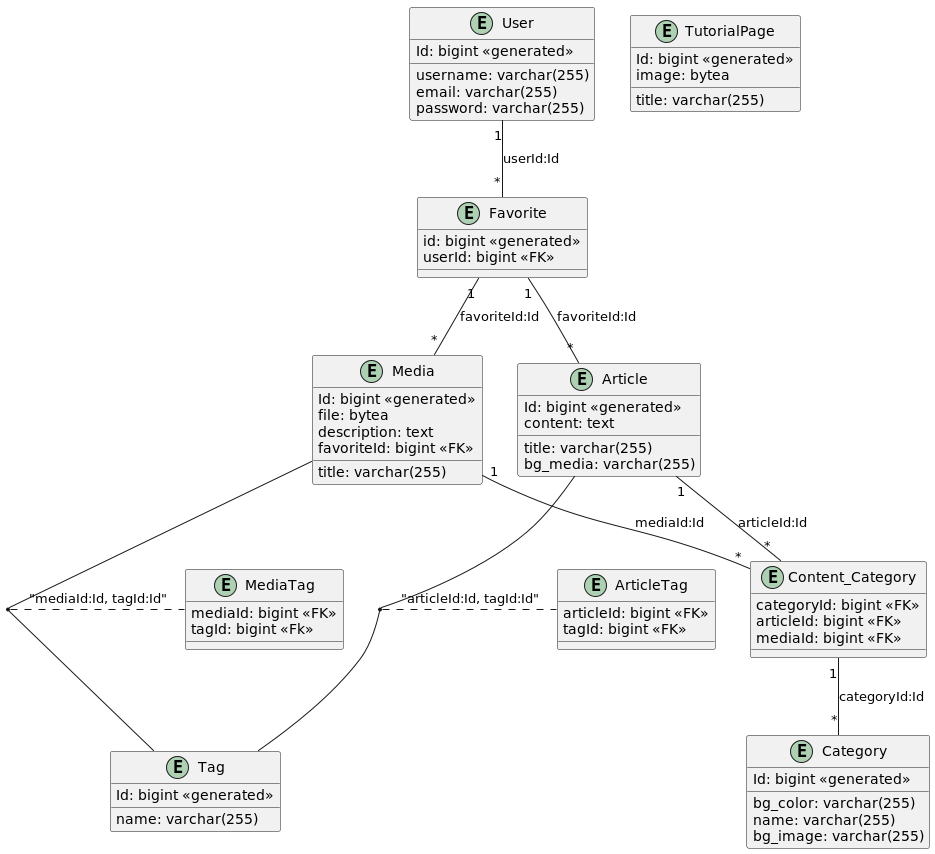
\includegraphics[height=1\textwidth]{./pics/erd.png}
    \caption{ERD}

  \end{figure}
\end{spacing}


\section{Medias und Articles}

Grundsätzlich haben wir als Team entschieden,
die Artikeln und die Medien in zwei speraten Tabellen zu speichern,
da Artikeln mehrere Bilder, Videos und Audios Inhalte enthalten können.
Diesen können dann mittels ein "Rich Text Editor" hinzugefügt werden.
Bei "Media" handlet es sich nur um ein Medienelement,
nähmlich ein Bild, Video oder Audio File. Es ist aber wichtig anzumerken,
dass keine Benutzeroberfläche für die Artikeln implementiert wurde, da der Kunde
diese nicht in dem \textbf{M}inimal \textbf{V}iable \textbf{P}roduct (MVP) haben wollte.
Für die Relaisierung des kompletten Datenmodels war aber das Einfügen der Artikel erforderlich.

\section{TutorialPage}
Die Entität "TutorialPage" hat keine Beziehungen zu anderen Entitäten, da sie nur für den Inhalt des Tutorial-Slideshows,
die nach der erfolgreichen Installation der App angezeigt wird, gedacht ist.

\begin{figure}[H]
  \centering
  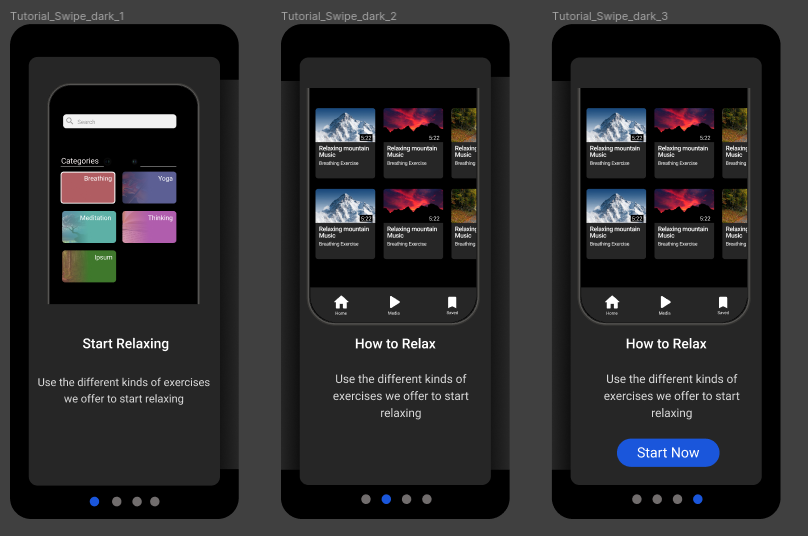
\includegraphics[height=0.5\textwidth]{./pics/slideshow.png}
  \caption{Screenshot aus dem UI Prototyp von Relaxoon}
\end{figure}

Mit der Persestierung der Inhalte von der Slideshow könnte die Erstellung
von neuen Builds bei jeder Änderung vermieden werden.


\section{Suche und Filterungen}

Bei den Filterungen wurde der "Interactive Query Builder" verwendet,
um die Filterparameter der Abfragen zu generieren
und diese dann bei den REST Abfragen anzuhängen.
Es gibt auch eine "Query Engine", welche die gleiche Funktion wie diese
"Interactive Query Builder" hat.
Diese kann in dem \textbf{O}bject \textbf{R}elational \textbf{M}apper (ORM) angewendet werden.
Mit der Verwendung dieser "Interactive Query Builder" kann man die Daten,
die man von den REST-Resourcen bekommt, anpassen.
Es gibt auch die Möglichkeit, die REST-Resource im Backend mittels dieser
"Query Engine" anzupassen.
Allerdings wurde diese "Query Engine" nicht verwendet,
da die Dokumentation bzw. Intellisense von dem ORM sehr ungenau war.

\begin{figure}[H]
  \centering
  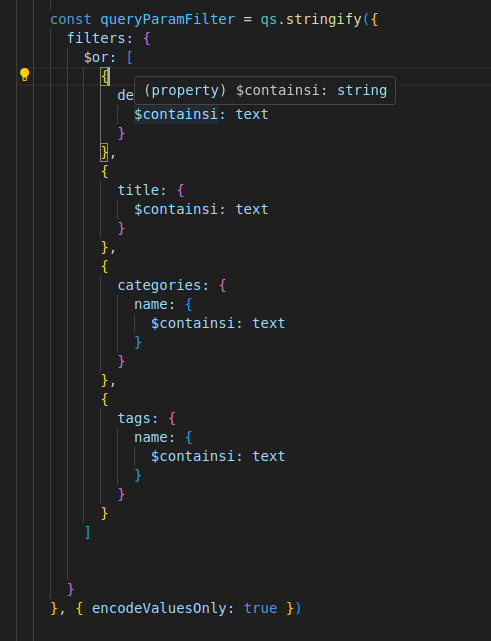
\includegraphics[ width=1\textwidth]{./pics/query-builder.png}
  \caption{Beispiel für den Interactive Query Builder}
\end{figure}




\begin{spacing}{1}
  \textbf{API-Route mit den angehängten generierten Abfrageparameter}:
  \newline
  \textcolor{red}{/medias?\&populate[tags]=true
  \&populate[file]=true
  \&populate[favorite][populate]=\newline users\_permissions\_user}
\end{spacing}



\section{Help und Info Screen}

Mit der Speicherung der Inhalten von den Ansichten ''Help'' und ''Info''  ist neues Build für das Frontend nicht mehr nötig.
Somit kann der Content-Manager mehrere Freiheiten haben.
Diese Inhalte wurden mit sogenannten ''Single Types'' persestiert.
Ein ''Single Type'' ist nichts anders als eine Tabelle, die nur eine Zeile enthält.
Bei einer Änderung des Werts von diesem ''Single Type'' wird diese eine Zeile aktualisiert.


\section{Deployment}

\subsection{Allgemeins}

Die Firmen Solivstas und Macolution wollten das Endpordukt auf ihrer eigenen
Infrastruktur deployen und die Anwendungen
als Docker-Images in den Container-Registries von denen speichern.
Da die genannten Firmen keine Zugriffsrechte für das Team organisiert haben,
war es für das Team schwierig, beim finalen Deployment mitzumachen. Das Team hat aber die Möglichkeit gehabt,
beim Deployment auf dem Stagingsystem mitzuhelfen, da die Software auf einem externen Service, nämlich
Firebase App Distribution, hochgeladen wurde.
Der Betreuer wurde ebensfalls informiert und er verlangte ein lokales Deployment für das Backend mittels ''Minikube'' sowie ein Live-Demo für die Applikation auf einem Emulator


\subsubsection{Container Registry}

\begin{quotation}
  ``
  A container registry is a repository—or collection of repositories—used to store and access container
  images. Container registries can support container-based application development,
  often as part of DevOps processes.
  Container registries can connect directly to container orchestration platforms like Docker and Kubernetes.
  ''
  \cite{container-registry}
\end{quotation}


\subsection{Deployment Diagram für das Dev System}

//TODO Deployment Diagram für Dev
\begin{figure}
  \centering
  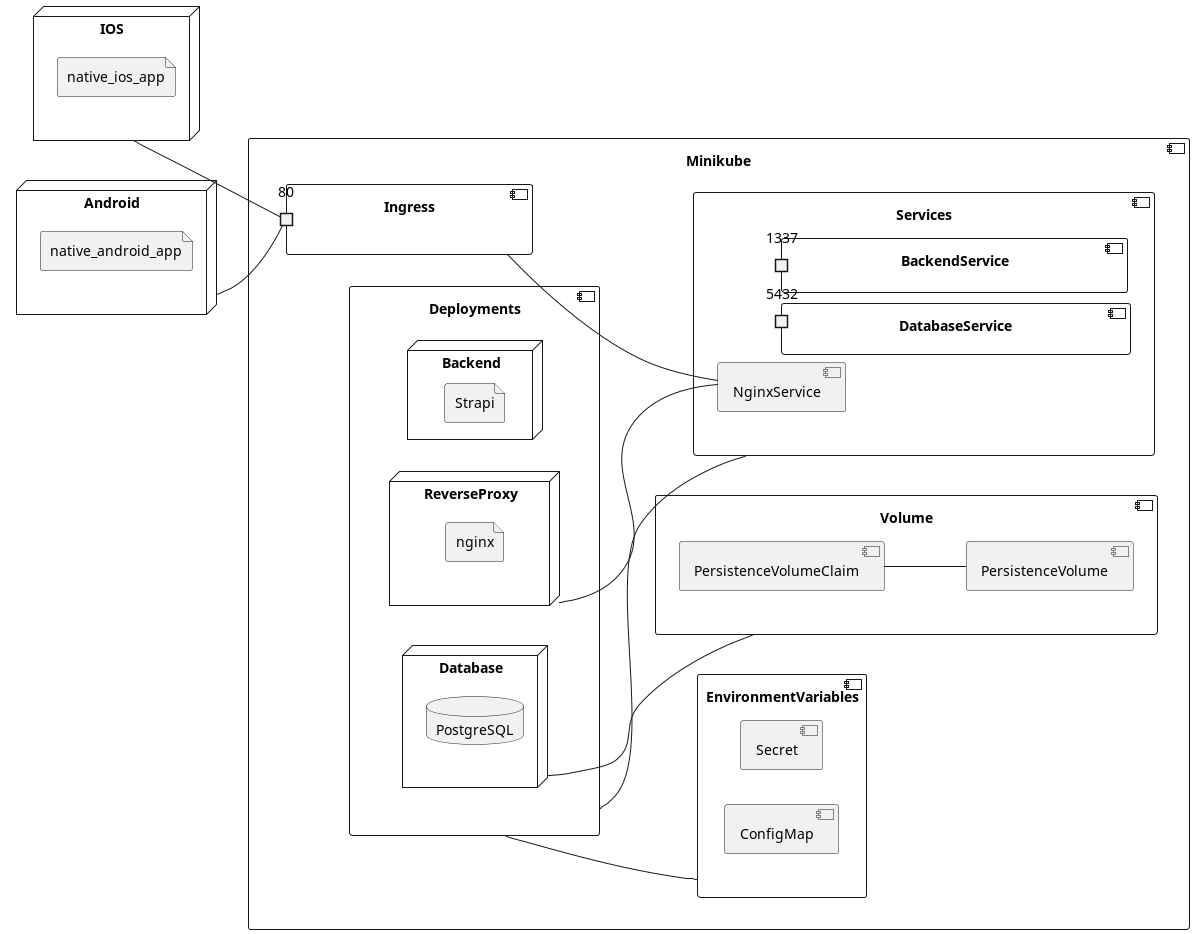
\includegraphics[width=\textwidth]{./pics/dev-deployment.png}
  \caption{Deployment für Dev System}

\end{figure}

\subsection{Deployment Diagram für das Staging System}


//TODO Deployment Diagram für Staging

\section{Buildprozess für das Frontend}

Damit man das Frontend deployt, muss man zuerst den nativen Android und IOS Code generieren.
Danach sollen die Android bzw. IOS Anwendungen mit einer IDE oder mit der Kommando-Zeile gebaut werden.
Um den nativen Code zu generieren ist folgendes einzugeben:
\begin{lstlisting}[language=Bash,caption=generate android and ios]
npx expo prebuild
\end{lstlisting}



\subsection{Erstellung einer .apk Datei}
Für Android wurde die .\textbf{A}ndroid \textbf{P}ac\textbf{K}age (apk)  mit dem Einsatz von gradle Wrapper generiert.
Foglendes muss installiert und richtig konfiguriert werden, damit  eine .apk Datei generierbar ist:



\begin{itemize}
  \item Java 11
  \item Installation von sdkmanager
  \item Lizenzen von sdkmanager müssen akzeptiert sein
  \item Installation von einer Android SDK
  \item Konfigurationen für JAVA\_HOME und ANDROID\_HOME
  \item Installation einer CLI namens "ninja"
\end{itemize}

Der Generierungsbefehl für die Build-Datei schaut dann wie folgendes aus:

\begin{lstlisting}[language=bash,caption=generate apk]
./gradlew assembleRelease
\end{lstlisting}



\subsection{Erstellung einer .ipa Datei}
Für IOS hat sich das Team entschieden, die App mit der mittels Xcode zu bauen, da die andere Variante nicht so einfach ist.


Es ist aber noch anzumerken, dass die nativen Libraries in der  Swift-Codebase eingebunden werden sollen.
Dafür ist dieser Befehl geeignet:
\begin{lstlisting}[language=bash, caption=bind ios libraries]
pod install
\end{lstlisting}


<Coming Soon>

\section{Deployment von dem Backend}


Dabei sind folgende Systemkomponenten zu betrachten:

\begin{enumerate}
  \item Die Datenkbank
  \item  Das Headless-CMS
  \item Nginx Reverse-Proxy
\end{enumerate}


\subsection{Pushen einer Anwendung auf ein Containerregister}

Für das Pushen einer Anwendung auf \textbf{G}it\textbf{H}ub \textbf{C}ontainer \textbf{R}egistery (GHCR), ist die Containerisierung der Anwendung notwendig.
Um Strapi zu containerisieren, wurde folgendes Dockerfile geschrieben

\begin{lstlisting}[caption=Strapi Dockerfile]
  # Creating multi-stage build for production
  FROM node:18-alpine as build
  RUN apk update && apk add --no-cache build-base gcc autoconf automake zlib-dev libpng-dev vips-dev git > /dev/null 2>&1
  ARG NODE_ENV=production
  ENV NODE_ENV=${NODE_ENV}
  
  WORKDIR /opt/
  COPY package.json package-lock.json ./
  RUN npm install -g node-gyp
  RUN npm config set fetch-retry-maxtimeout 600000 -g && npm install --only=production
  ENV PATH /opt/node_modules/.bin:$PATH
  WORKDIR /opt/app
  COPY . .
  RUN npm run build
  # Creating final production image
  FROM node:18-alpine
  RUN apk add --no-cache vips-dev
  ARG NODE_ENV=production
  ENV NODE_ENV=${NODE_ENV}
  ENV HOST=0.0.0.0
  ENV PORT=1337
  ENV APP_KEYS=secret
  ENV API_TOKEN_SALT=secret
  ENV ADMIN_JWT_SECRET=secret
  ENV TRANSFER_TOKEN_SALT=secret
  # Database
  
  # Database
  ENV DATABASE_CLIENT=postgres
  ENV DATABASE_HOST=localhost
  ENV DATABASE_PORT=5432
  ENV DATABASE_NAME=strapi
  ENV DATABASE_USERNAME=strapi
  ENV DATABASE_PASSWORD=strapi
  ENV DATABASE_SSL=false
  ENV JWT_SECRET=cVRog3q5woTNB8EJ+vKPFA==
  
  
  
  
  WORKDIR /opt/
  COPY --from=build /opt/node_modules ./node_modules
  WORKDIR /opt/app
  COPY --from=build /opt/app ./
  ENV PATH /opt/node_modules/.bin:$PATH
  
  RUN chown -R node:node /opt/app
  USER node
  EXPOSE 1337
  CMD ["npm", "run", "start"]
    
\end{lstlisting}





Danach soll ein Docker-Image aus diesem File generiert werden und dieses in dem folgenden Format getagt werden:
\newline
ghcr/\textbf{<Name des Users oder der Organisation>}/\textbf{<Name des Images>}:\textbf{<Version>}
\newline
Damit das Image jetzt auf GHCR gepusht werden kann, ist das Einloggen in diesem erforderlich.
Danach kann die Anwendung auf GHCR veröffentlicht werden.
Alle benötigten Befehle für diesen Kapitel sind im folgenden Code-Snippet zu finden:

\begin{lstlisting}[language=bash,caption=Veröffentlichung eines Docker-Images auf GHCR]
docker build -t relaxoon-strapi .
docker tag relaxoon-strapi ghcr.io/Abdulrahman-AL-Sabagh/relaxoon-strapi:latest
docker login ghcr.io
cat ./token.txt | docker login --username Abdulrahman-AL-Sabagh --password-stdin
docker push ghcr.io/Abdulrahman-AL-Sabagh/relaxoon-strapi:latest
    
\end{lstlisting}
\cite{upload-to-ghcr}


\subsection{Erstellung von einer Deployment-Komponente}

Eine Deployment-Komponente dient dazu, dass ein Pod erstellt wird und die benötigten Resourcen bzw. Volumes und Zugriffsrechten
dafür definiert werden.\cite{k8s-deployment}

Für das Anlegen einer Deployment-Komponente muss man zuerst die Anwendung containerisieren.
Für weit verbreitete Software wie z.B.: PostgreSQL gibt es bereites viele vorhandene Images auf unterschiedliche Container-Registries

Folgende Befehle wurden verwendet, um die Deployment-Komponenten für Strapi und PostgreSQL zu erstellen:

\begin{lstlisting}[language=bash, caption=create k8s deployments]
kubectl create deployment relaxoon-db --image=postgres:12.16-bullseye --port=5432
kubectl create deployment relaxoon-strapi --image=ghcr.io/Abdulrahman-AL-Sabagh/relaxoon-strapi:latest --port=8080
    
\end{lstlisting}


\subsubsection{Was ist ein Pod}

\begin{quotation}
  ``
  Ein Pod (übersetzt Gruppe/Schote, wie z. B. eine Gruppe von Walen oder eine Erbsenschote)
  ist eine Gruppe von einem oder mehreren Containern mit gemeinsam genutzten Speicher- und
  Netzwerkressourcen und einer Spezifikation für die Ausführung der Container.
  Die Ressourcen eines Pods befinden sich immer auf dem gleichen (virtuellen) Server,
  werden gemeinsam geplant und in einem gemeinsamen Kontext ausgeführt.
  Ein Pod modelliert einen anwendungsspezifischen "logischen Server": Er enthält eine oder mehrere
  containerisierte Anwendungen, die relativ stark voneinander abhängen.
  ''
  \cite{pod}
\end{quotation}






\subsection{Erstellung einer Service-Komponente}

Mit dem Einsatz eines Services in Kubernetes können Pods,
die sich im gleichen Cluster befinden,miteinander kommunizieren. \cite{k8s-service}

Für das Anlegen einer Service-Komponente kann man diesen Befehl nutzen:

\begin{lstlisting}[language=bash,caption=create a service component]
kubectl expose deployments/<Name des Pods> --port=5432
\end{lstlisting}



\subsection{Erstellung einer Persistence-Volume-Komponente}

Die Sogennanten \textbf{P}ersistence-\textbf{V}olumes (PV) dienen dazu, dass keine Datenverluste entstehen, wenn ein Pod gestoppt oder gelöscht wird.
Folgende Konfigurationen wurden die Generierung dieser Komponente verwendet

\begin{lstlisting}[caption=PV.yml]
apiVersion: v1
kind: PersistentVolume
metadata:
  finalizers:
  - kubernetes.io/pv-protection
  labels:
    type: local
  name: relaxoon-pv
  resourceVersion: "33077"
  uid: ae6d772a-0090-4074-b3ac-1edb929daf29
spec:
  accessModes:
  - ReadWriteOnce
  capacity:
    storage: 10Gi
  hostPath:
    path: /mnt/data
    type: ""
  persistentVolumeReclaimPolicy: Retain
  storageClassName: manual
  volumeMode: Filesystem
status:
  phase: Available    
    
\end{lstlisting}


\subsection{Erstellung einer Persistence-Volume-Claim-Komponente}

Damit der Pod auf die Persistence-Volume-Komponente zugreifen kann, ist die Verwendung von
sogenannten \textbf{P}ersistence-\textbf{V}olume-\textbf{C}laims (PVC) notwendig.

Dafür wurden folgende Konfigurationen verwendet

\begin{lstlisting}[caption=PVC.yml]
apiVersion: v1
kind: PersistentVolumeClaim
metadata:
  finalizers:
  - kubernetes.io/pvc-protection
  name: relaxoon-pvc
  namespace: default
spec:
    accessModes:
      - ReadWriteMany
    resources:
      requests:
        storage: 10Mi
    storageClassName: standard
    
\end{lstlisting}


\subsection{Umgebungsvariablen in Kubernetes}
Es gibt drei Methoden, um eine Umgebungsvariable in Kubernetes zu definieren.

\begin{itemize}
  \item Man definieren diese in der Deployment-Komponente
  \item Man verwendet eine Secret-Komponente
  \item Man verwendet eine ConfigMap-Komponente
\end{itemize} \cite{envs-k8s}

Für die Credentials von PostgreSQL und die Token der API wurde eine Secret-Komponente verwendet, da diese solche Daten entschlüsselt.
Für die restlichen Umgebungsvariablen war eine ConfigMap nötig, da die Anzahl der restlichen Variablen nicht gering war. \cite{secrets}

\subsubsection{ConfigMap}

\begin{quotation}
  ``
  A ConfigMap is an API object used to store non-confidential
  data in key-value pairs. Pods can consume ConfigMaps as environment variables,
  command-line arguments, or as configuration files in a volume.
  \cite{config-maps}
  ''
\end{quotation}
//TODO Befehl für Secrets noch hinzufügen
//TODO Config für ConfigMap noch hineingeben

\subsection{Erstellung einer Ingress-Komponente}

Damit der Emulator, der sich außerhalb des lokalen Clusters von Minikube befindet,
mit dem deployten Backend kommunizieren kann,
ist das Anlegen einer Ingress notwendig.

//TODO Config für die Ingress-Komponente noch hingeben

//TODO Dieses Kapitel noch fertigschreiben



//TODO über Reverse-Proxy noch schreiben


\section{Hochladen einer Mobileapp auf Firebase App Distribution}

Nachdem Anlegen eines Accuonts bei Firebase sind folgende und die Erstellung eines Projektes Schritte zu machen:


\begin{figure}
  Damit die benötigten Firebase Services für die Applikationen aktiviert werden, muss man zuerst die benötigten Konfigurationen eingeben.
  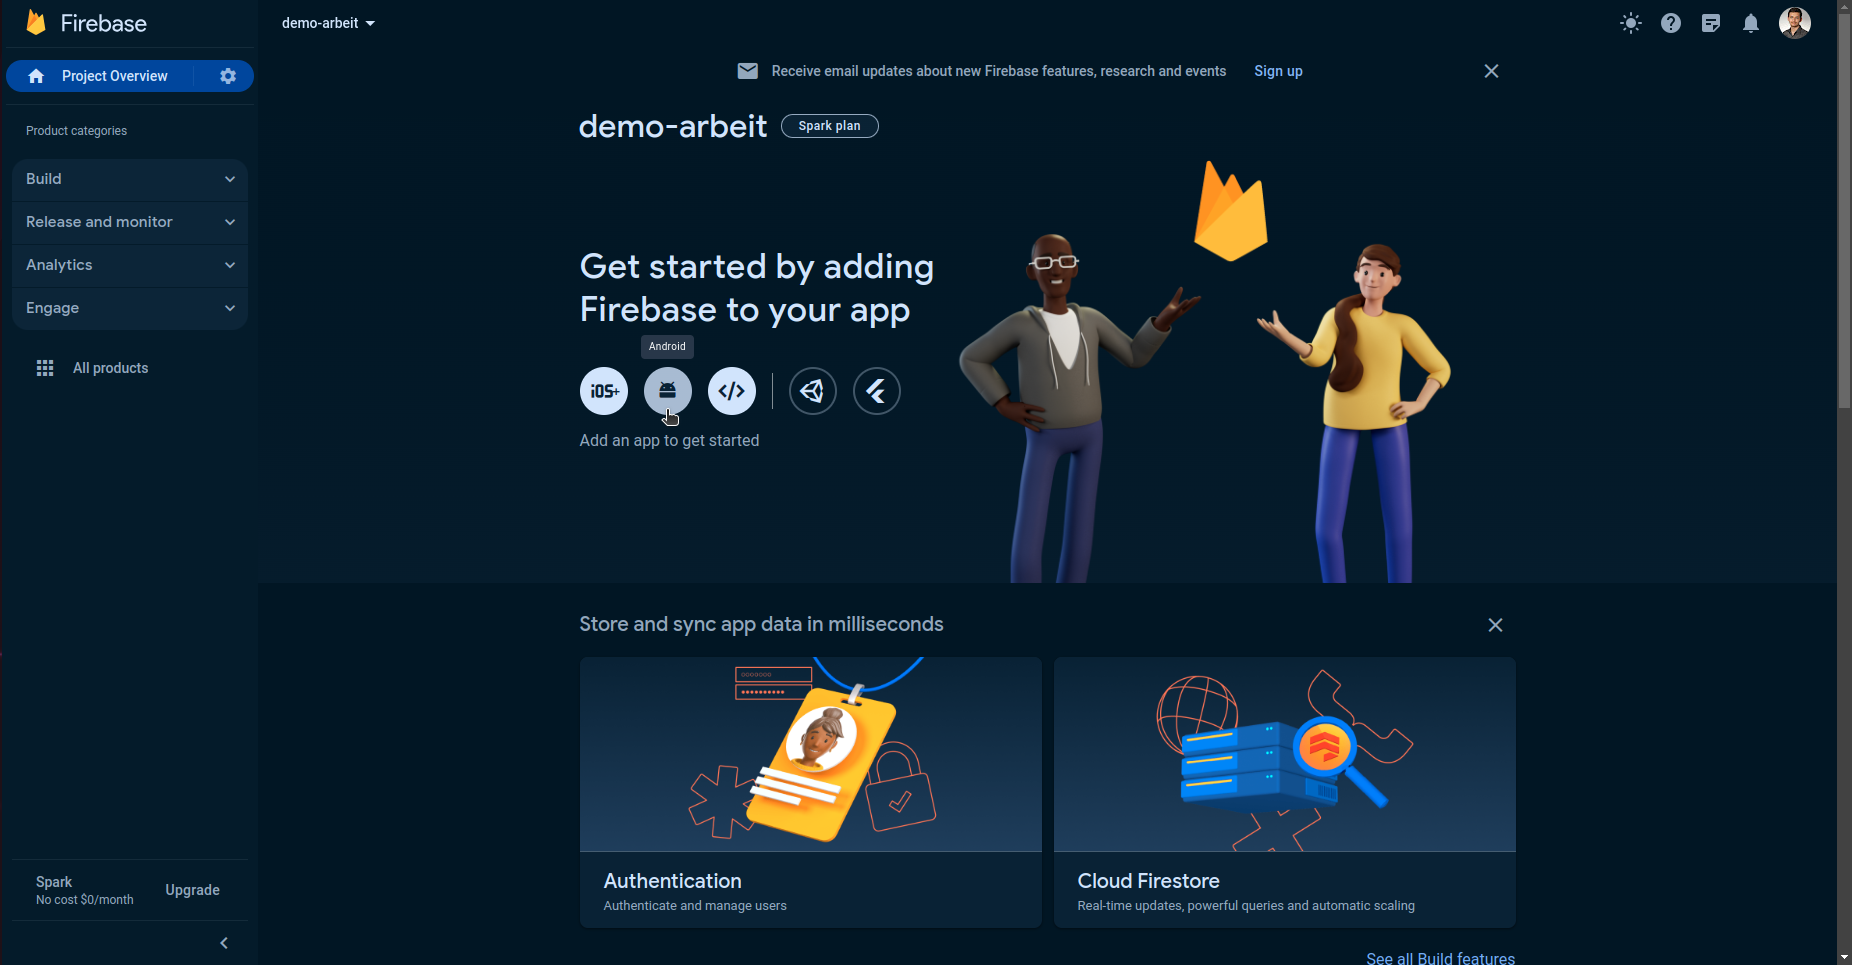
\includegraphics[width=\textwidth]{./pics/firebase1.png}
  \caption{create android config}
\end{figure}



\begin{figure}
  Folgende Daten müssen eingegeben werden, damit die Firebase Services für die Android Applikation eingeschaltet werden können.

  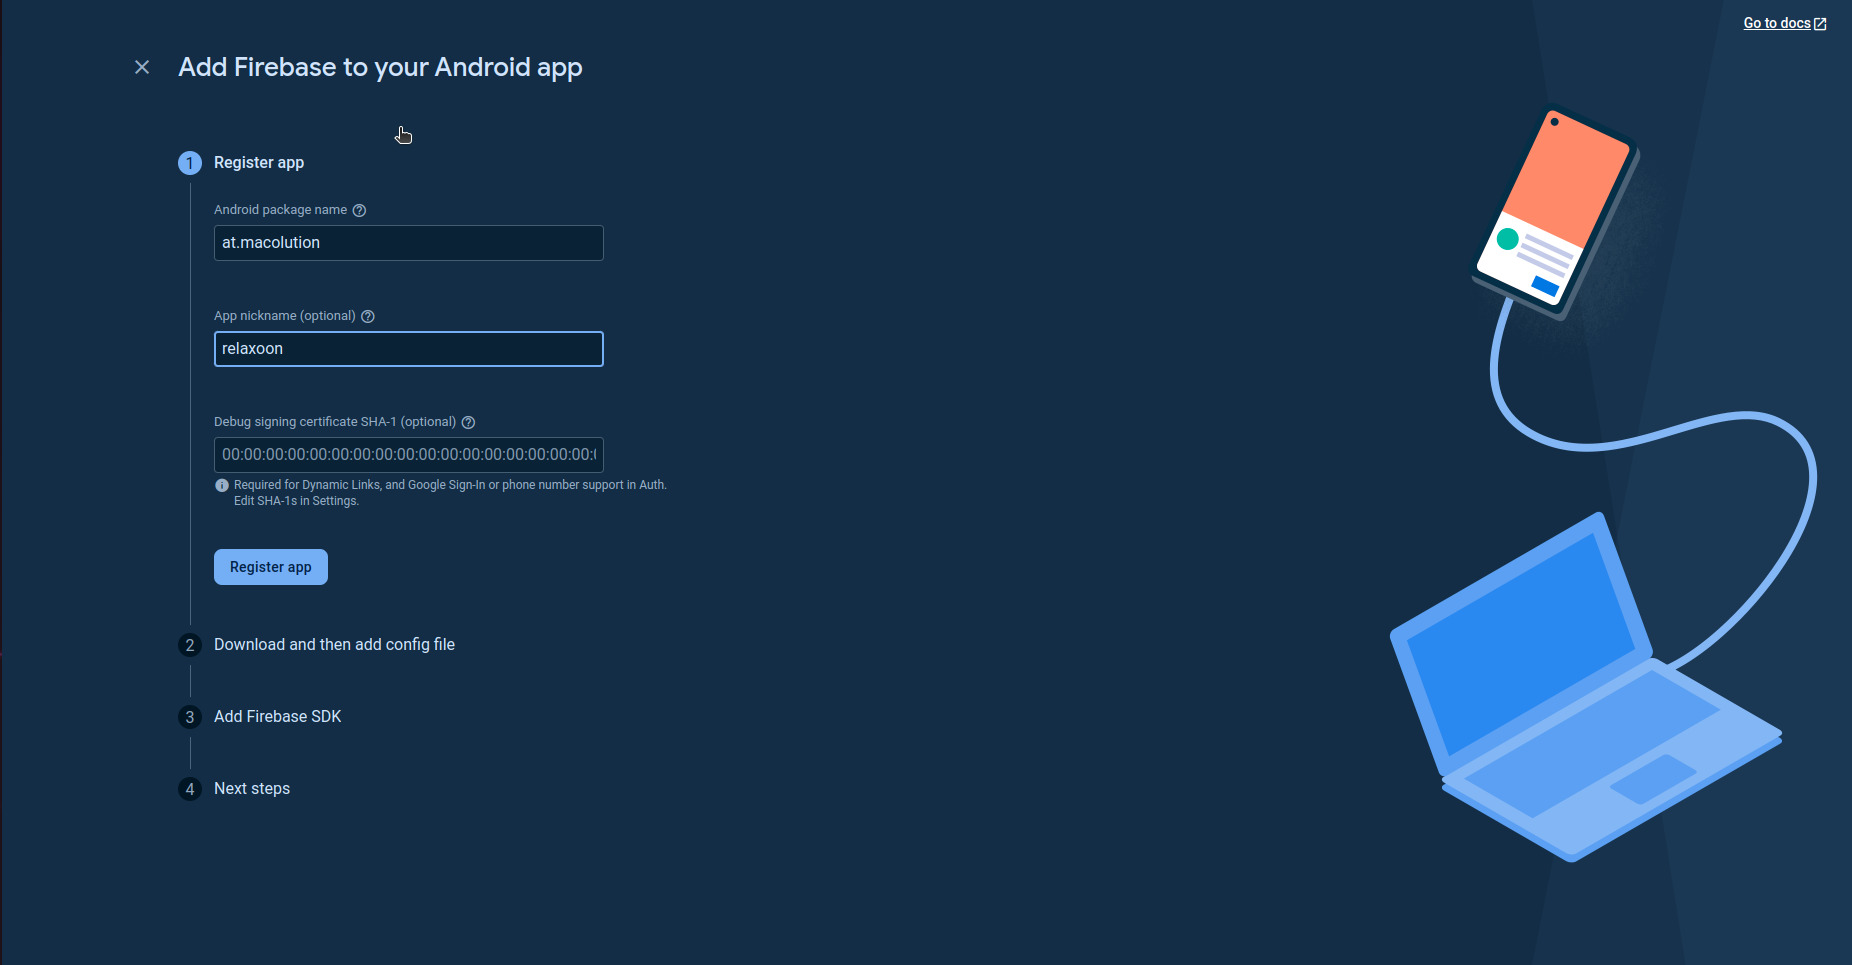
\includegraphics[width=\textwidth]{./pics/firebase2.png}
  \caption{Android Config}
  Die restlichen Punkte sind für das Projekt Relaxoon irrelevant,
  da die Firebase-SDK in der vorleigende Arbeit nicht eingesetzt wird.
\end{figure}



\begin{figure}
  Danach soll man  auf die App Distribution gehen und dann auf ''Get Started'' klicken
  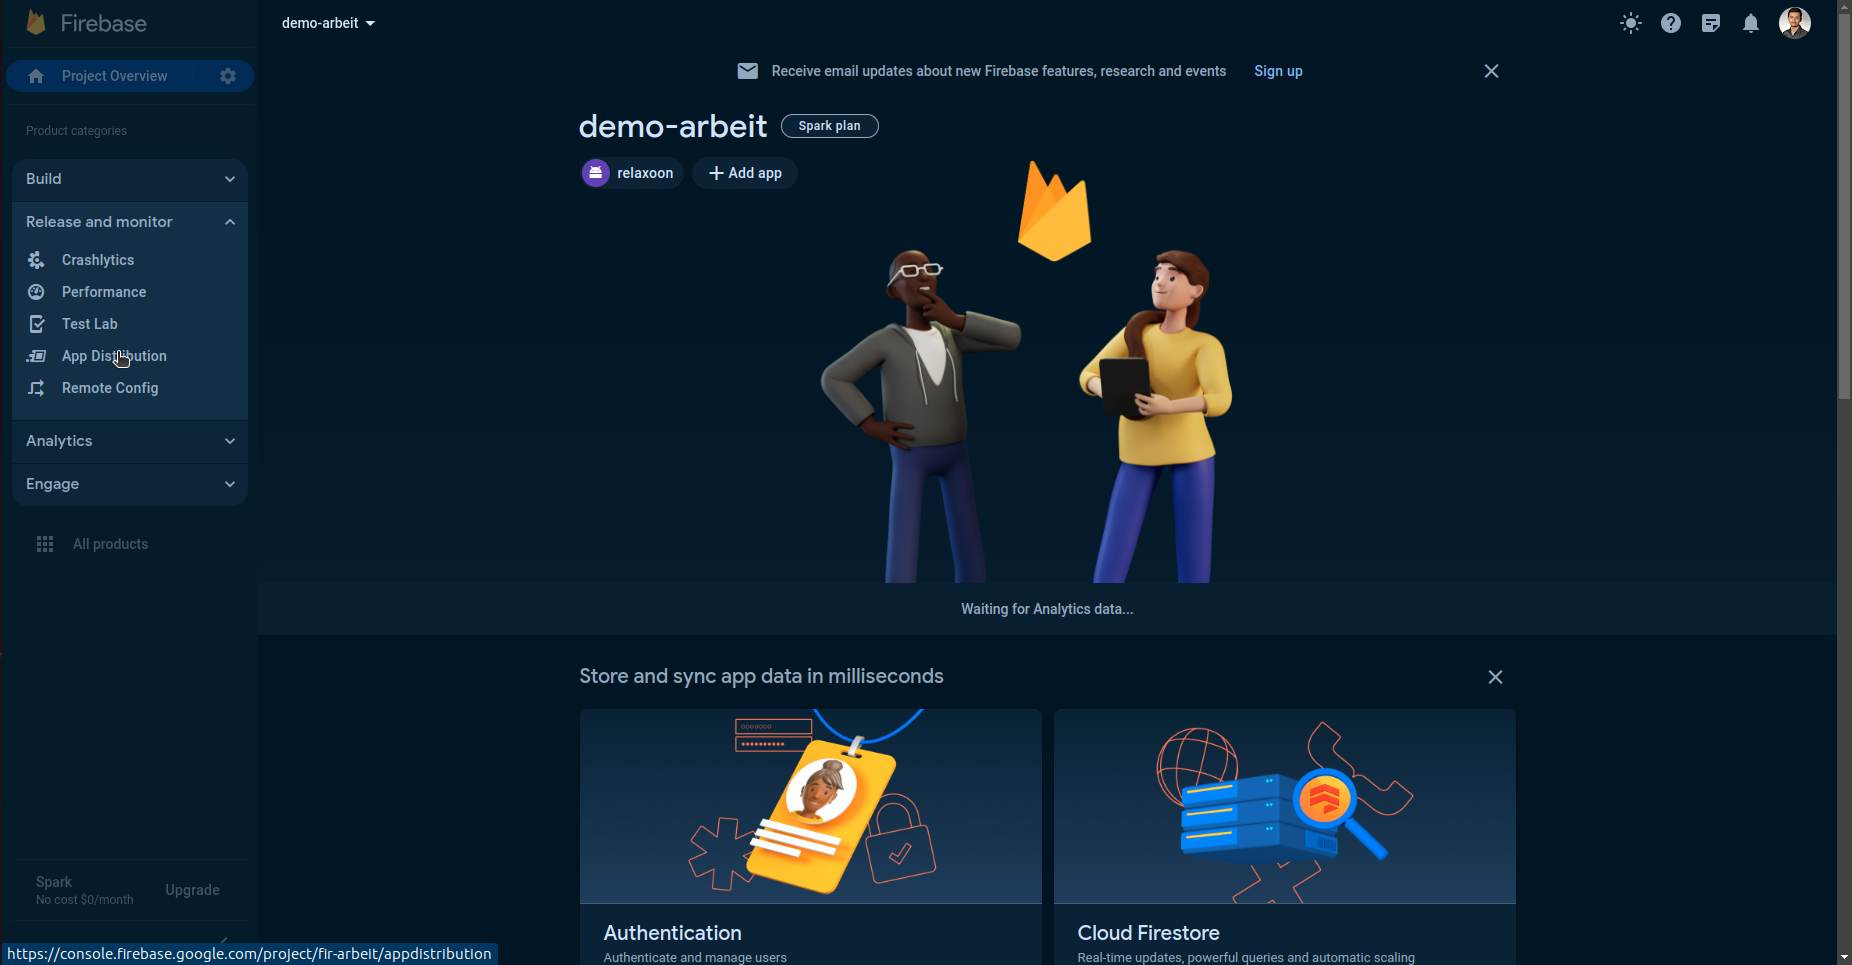
\includegraphics[width=\textwidth]{./pics/firebase3.png}
  \caption{App Distribution}
\end{figure}

\begin{figure}
  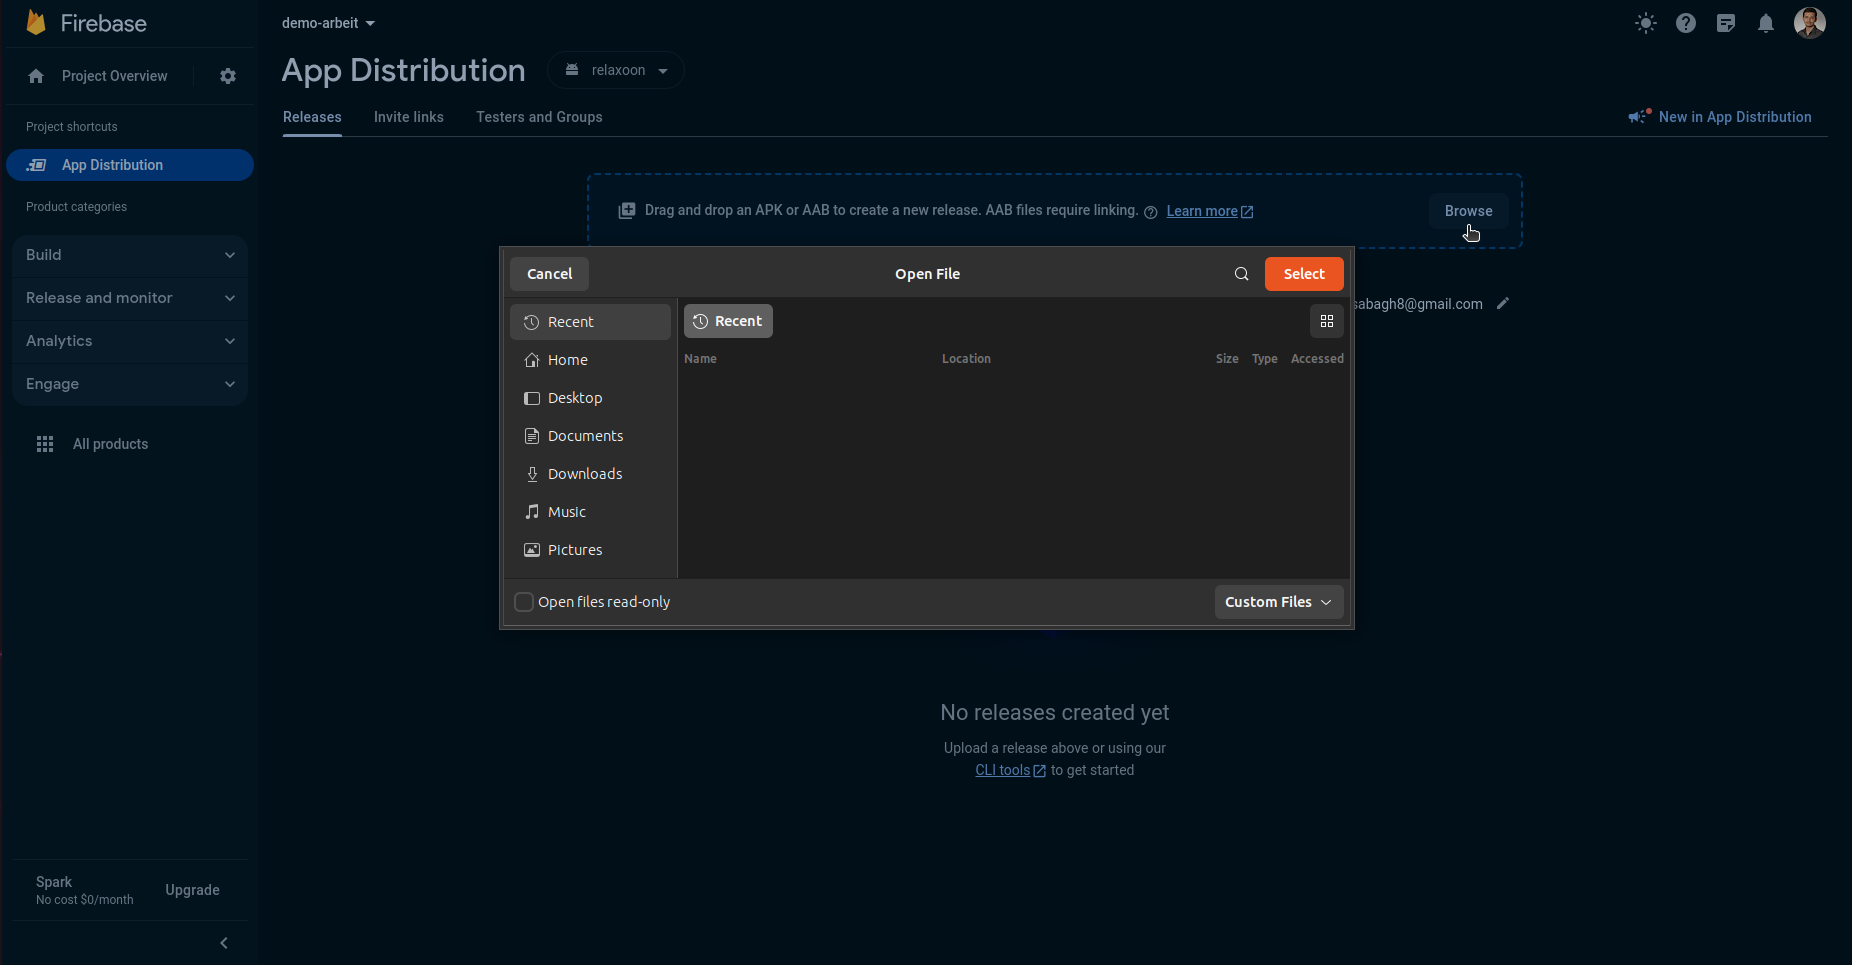
\includegraphics[width=\textwidth]{./pics/firebase4.png}
  \caption{App upload}
  Die App kann mit diesem ''Browse Fenster'' oder mit ''Drag and Drop'' hochgeladen werden

\end{figure}



\begin{figure}
  Das Produkt kann dann an anderen TestUsers verteilt werden, indem man die Email-Adressen dieser Testers beim Release eingibt.
  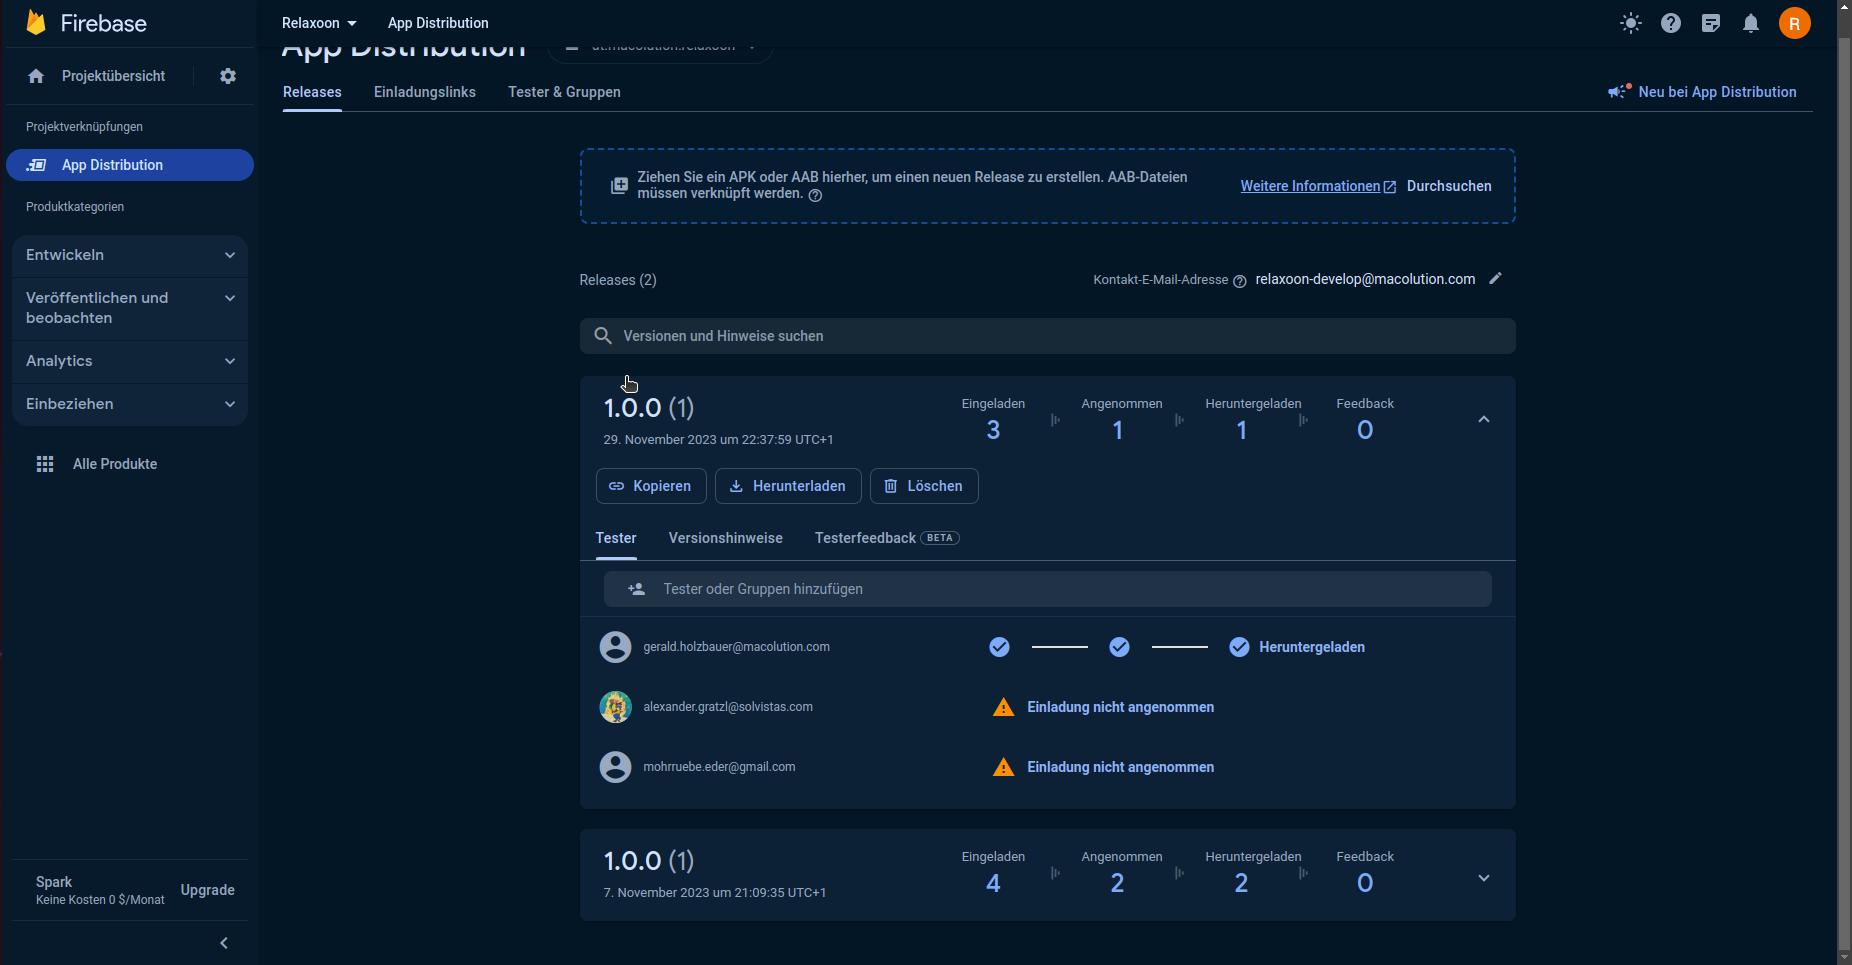
\includegraphics[width=\textwidth]{./pics/firebase5.png}
  \caption{releases}
\end{figure}

